\section{Background}
\label{background}

% presentar las siguientes subsecciones

% intro a que ahora se va a hablar de soluciones IoT que usen semántica
% Having analyzed non-specific solutions for distributed semantic architectures, the next step is to evaluate the use of semantics from the \ac{iot} perspective.

% \label{sec:sw_providers}

% La acepción de Name resolution cambia depende del contexto!
% http://en.wikipedia.org/wiki/Name_resolution

% Name resolution vs recognition
% http://stackoverflow.com/questions/8589005/difference-between-named-entity-recognition-and-resolution



\subsection{Sharing Semantic Knowledge in Peer-to-peer}
The problem of sharing semantic knowledge distributedly has gained attention since the first steps of the Semantic Web \citep{berners-lee_semantic_2001}.
Multiple architectures from the \emph{Peer-to-peer} (P2P) communication model have been used \citep{filali2011survey}.
The P2P architectures are commonly categorized as \emph{unstructured}, \emph{structured}, and \emph{hybrid}.

% Parte del de P-Grid, parte de la survey
% RDFS+ de zhou del 2010 (este es el que clasifica trabajos como de un tipo u otro)
% muhleisen2011survey
% Cuidado: llaman a los protocolos de gossiping epidemic por su forma de propagar consultas
\noindent\textbf{Unstructured.}
In this category, the peers are unaware of the resources stored by other peers.
Therefore, the connections between the peers are based on randomized approaches.
The simplest solution is using flooding \citep{halevy_piazza:_2003,krummenacher_open_2009} which broadcasts every query to all peers to obtain high accuracy.
Other solutions restrict the broadcast by using random routing which leads to less accurate results.
Both cases are inefficient and do not scale well.
To reduce the negative effects of randomness, \citet{zhou_building_2009} uses metadata of neighbor nodes to route the queries and reorganize the topology. % in S-RDF
Interestingly, our solution also uses metadata from other nodes.
However, we do not focus on the network layer and therefore, we do not change the topology.
In contrast, we change the duties of the nodes according to their capabilities.
% edutella al ppio (luego paso a ser super-peers)

% Parte este discurso está sacado de la intro de "P-Grid: A Self-organizing Structured P2P System"
% Otro ejemplo sería swarm-based
\noindent\textbf{Structured.}
In this category, the peers  maintain information about the resource of other peers.
The most common solutions are those based on distributed hash tables (DHT).
DHT solutions calculate the hash functions over the content which needs to be stored or retrieved.
Using this hash, one can know who is the peer in charge of managing this particular content.
% link con lo de arriba
Consequently, the queries can be directed to the appropriate peers generating fewer messages.
Unfortunately, peers joining or leaving these systems result in expensive restructuraction operations.
This maintenance cost makes this solution impractical for networks with high peer mobility (e.g., the \ac{iot}).
In addition, the hash function does not consider the different capabilities for the peers.
For example, we have to control the storage and the battery of small devices.
% What if a limited device exhausts its storage or faces much more requests than a powerful server?
% zhou2009 también defiende lo mismo
% "We believe that an unstructured P2P paradigm can better model our collaborative scenario in which peers maintain
% their triples and share them with others."
% "We recognize and respect the rights of individuals to maintain their own data, which precludes highly scalable
%  techniques such as DHTs."
% Otras razones de peso defendidas en la intro: freshness, dependencia de otros
Some examples of DHT-based solutions are
RDFPeers \citep{cai_rdfpeers:_2004},
GridVine \citep{cudre-mauroux_gridvine:_2007},
TripCom\footnote{TripCom (IST-4-027324-STP, www.tripcom.org)}
% ellos lo consideran semi-descentralizado y los kernels funcionan por DHT
or one of the two architectural solutions proposed by SQPeers \citep{kokkinidis_query_2006}.
% otras aproximaciones como en uso de Semantic Overlay Networks, swarm-based (ignorar para aclarar el hilo)
% AG: estas son las más susceptibles de cambiar!

\noindent\textbf{Hybrid.}
Finally, the \emph{hybrid} architectures differentiate between a set of peers so-called super-peers in charge of complex tasks and the common ones.
The super-peers are usually connected through structured networks while the normal peers rely on any of those super-peers to perform tasks (e.g., query routing).
Edutella \citep{nejdl_super-peer-based_2003} and the second solution proposed by SQPeers \citep{kokkinidis_query_2006} are two examples of hybrid architectures.

\noindent\textbf{Our approach.}
% nos apoyamos en los super-peers sin dejar de tener nodos independientes (una vez tienen las clues)
% porque nosotros nos hemos decantado por esto? comparar con otras categorias y con soluciones de su categoría.
Following this categorization, our solution is a hybrid architecture since some of the nodes in our architecture have special responsibilities.
In particular, we use intermediaries which store what Edutella and SQPeers call indices.
The main difference with these solutions is that the intermediary role is not fixed. % as with other super-peers.
Instead, the nodes dynamically decide which one should intermediate according to their energy autonomy and capacities.
Thus, we aim to ease the deployment of our solution and make it flexible and able to adapt to multiple scenarios.
At the same time, the most powerful (i.e. energetically and in computing power) devices can support those that are resource constrained.


% Estas han pasado al estado del arte
%\subsection{Semantics in the \acl{iot}}
%\subsection{Semantics in the \acl{wot}}



% ¿Mereceria la pena rescatar el porque DNS no se puede usar sin mas en nuestro caso?
% Yo lo he quitado creyendo que NO por:
%      - Simplificar y no enmarañar mas el discurso.
%      - Es una cosa que me parece basica si se comprende el problema.

% Most \ac{wot} solutions, use DNS-based discovery to locate the REST services \emph{Providers} \cite{ishaq_facilitating_2012}.
% In semantic \ac{wot}, the use of DNS-based discovery arises as a solution to locate the device holding the response for a specific request.
% Providing that the query already includes the URL of the host that contains the requested information (see Figure \ref{fig:triple}),
% we could easily locate such device using standard network protocols.
% Unfortunately, this does not always apply to Semantic Web for two reasons:
% \begin{enumerate}[(a)]
%  \item sometimes URIs are not URLs and therefore, they cannot be used as locators but just as identifiers.
%  \item the nature of the semantic web encourages to link concepts, so the same URI may be included in multiple graphs
% stored in different devices.
% \end{enumerate}
% Therefore, any DNS-based resolution strategy should be used only as a complementary mechanism for our clue-based solution.
% 
% \begin{figure}
% \centering
% 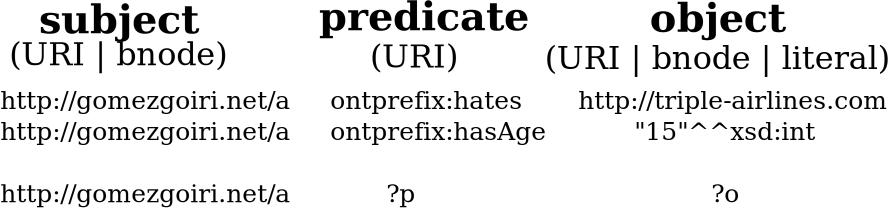
\includegraphics[width=0.8\columnwidth]{./img/RDFTriple/RDFTriple.pdf}
% \caption{Basic composition of a RDF triple, two examples and a wildcard based template where both examples match.
% \textit{ontprefix} is an alias, known as prefix in most
% Semantic languages, for the beginning of an URI.}
% \label{fig:triple}
% \end{figure}
% 
% Without a DNS-based system, we need to share enough information with the \emph{Consumers} to deduce the relevant \emph{Providers}.
% At the same time, according to the resource constrained devices needs, we want to avoid sharing too much information between the nodes.
% This results in a conflict of interests which should be solved with a trade-off. % IG: esta frase es la descripcion de un trade-off en si